\documentclass{beamer}
%
% Choose how your presentation looks.
%
% For more themes, color themes and font themes, see:
% http://deic.uab.es/~iblanes/beamer_gallery/index_by_theme.html
%
\mode<presentation>
{
  \usetheme{NYU}      % or try Darmstadt, Madrid, Warsaw, ...
  \usecolortheme{default} % or try albatross, beaver, crane, ...
  \usefonttheme{default}  % or try serif, structurebold, ...
  \setbeamertemplate{navigation symbols}{}
  \setbeamertemplate{caption}[numbered]
} 
\usepackage{listings} 
\usepackage{bera} 

\usepackage[ruled]{algorithm2e}

\usepackage{dsfont}
\usepackage[export]{adjustbox}



\usepackage{MnSymbol}%
\usepackage{wasysym}%

\usepackage{booktabs} 

\usepackage[english]{babel}
\usepackage[utf8x]{inputenc}

\title[Evolutionary Function Approximation for Reinforcement Learning]{Evolutionary Function Approximation for Reinforcement Learning}
\author{Yunian Pan}
\institute{ECE department}
\date{May. 10th 2019}
\titlegraphic{\hfill
\includegraphics[height=1.5cm]{nyu_stacked_color}}

\begin{document}

\begin{frame}{Reinforcement Learning Project}
  \titlepage
\end{frame}

% Uncomment these lines for an automatically generated outline.
%\begin{frame}{Outline}
%  \tableofcontents
%\end{frame}

\section{Outline}

\begin{frame}{Evolutionary Function Approximation for Reinforcement Learning}
\begin{block}{Outline:}
\begin{itemize}
  \item Some Background
  \item Methods and Results
  \item Experiments
  \item Conclusion
\end{itemize}
\end{block}
\vskip 1cm

\begin{block}{}
  In a word, DQN(Deep Q-Learning) + NEAT(Neuroevolution of augmenting topologies)
 \end{block}

\end{frame}

\section{Background}

\subsection{Q-Learning with NN}
\begin{frame}{}
  \footnotesize
  \begin{algorithm}[H]
    \scriptsize
    \caption{Q-Learning}
    \KwIn{$S:$ set of all states; $A:$ set of all actions; $\sigma:$ standard deviation of initial weights; 
    $c:$ output scale; $\alpha:$ learning rate; $\gamma:$ discount factor; $\lambda:$ eligibility decay rate; 
    $\epsilon_{td}:$ exploration rate; $e:$ total number of episodes;}
    \textbf{Initialize:} $N \leftarrow INIT-NET(S,A,\sigma)$ \;    
    \For{ $i \leftarrow 1 $ to $e$ }{$s, s^{\prime} \leftarrow $ null, INIT-STATE($S$)\;
    \While{Terminal-state(s)}{
      $Q[] \leftarrow c \times $$EVAL-NET(N,s^{\prime})$\;
      \textbf{With-prob}($\epsilon_{td}$) $a^{\prime} \leftarrow RANDOM(A)$\;
      \textbf{else:} $a^{\prime} \leftarrow \arg\max Q[j]$\;
      \eIf{$s \neq null $}
      {$BACKPROP(N,s,a,(r + \gamma \max_{j} Q[j])/ c, \alpha, \gamma, \lambda)$ \;}
      {$s, a \leftarrow s^{\prime}, a^{\prime}$\;
      $r, s^{\prime} \leftarrow TAKE-ACTION(a^{\prime})$}
    }
    }
    \end{algorithm}

  
\end{frame}


\subsection{NEAT}

\begin{frame}{Genetic Algorithm}
\begin{figure}[htbp]
  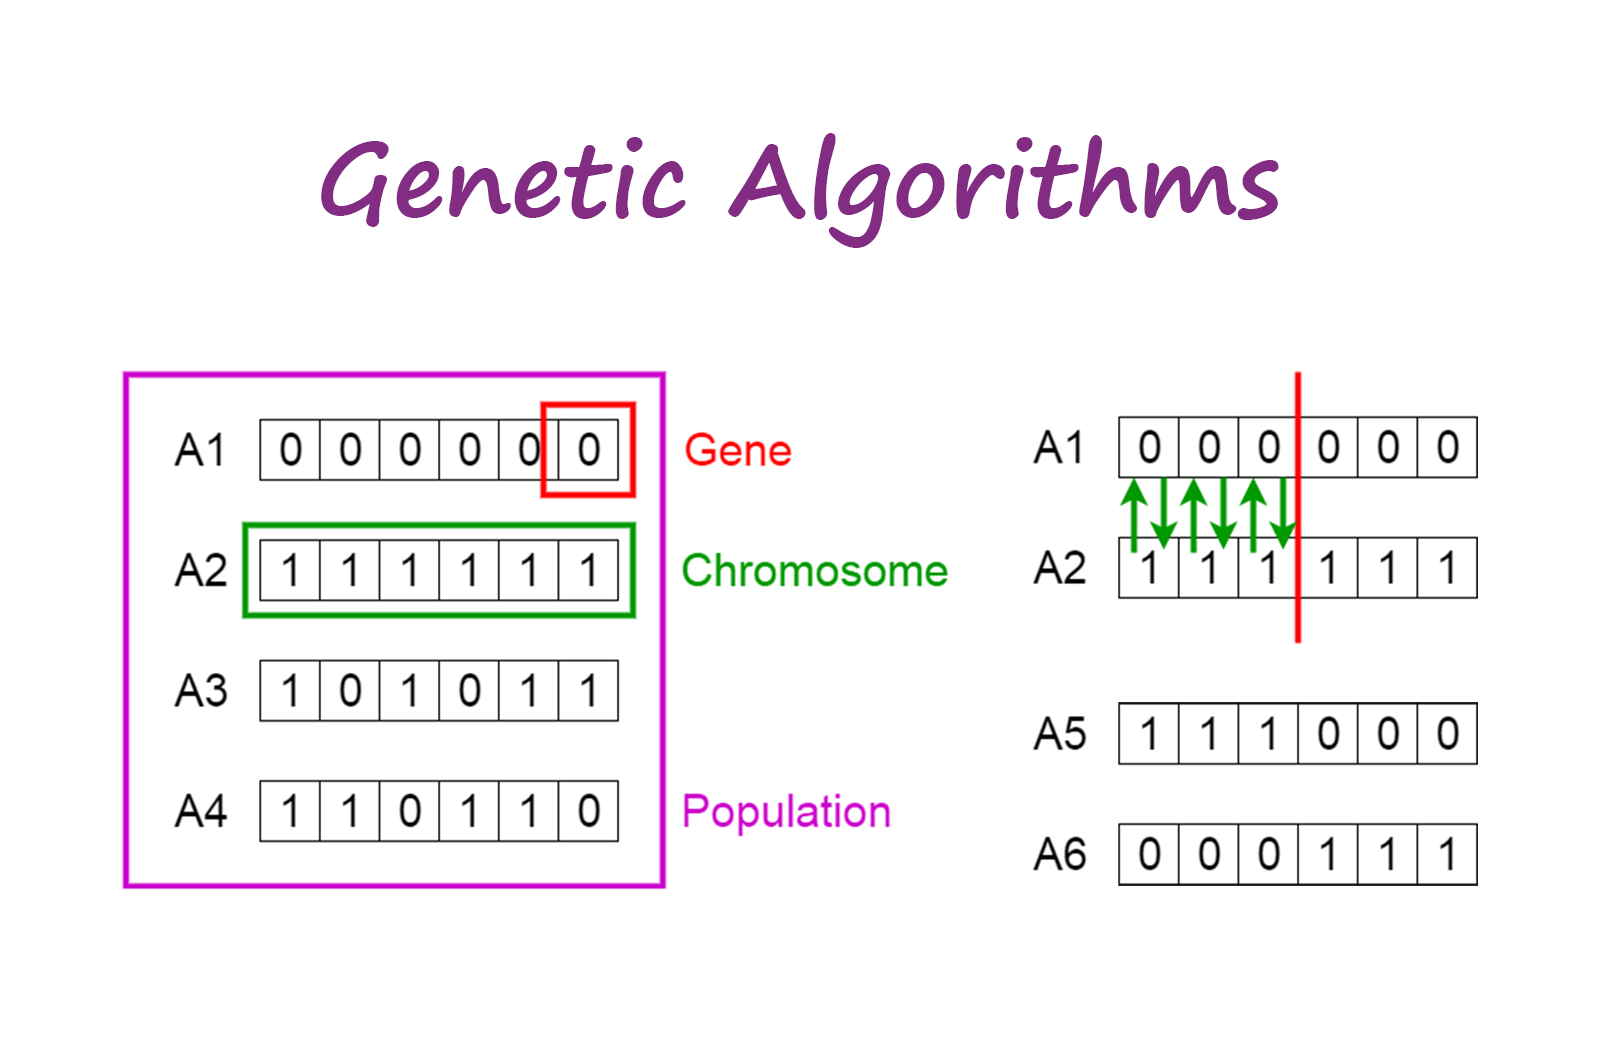
\includegraphics[width = .8\textwidth]{illu}
  \caption{Illustration from Google image}
\end{figure}
\end{frame}

\begin{frame}{Genetic Algorithm}
\begin{block}{}
  Standard evolution framework:
\begin{itemize}
  \item[(1)] Initialize population
  \item[(2)] Evolve from $1, \ldots, n_{generation}$:
  \begin{itemize} 
  \item[a)] Select from population according to \underline{fitness}
  \item[b)] Generate offspring through \underline{crossover} and \underline{mutation}
  \item[c)] Replace population with offspring. 
  \end{itemize}
\end{itemize}

\end{block}


\end{frame}
\begin{frame}
\begin{figure}[htbp]
  \includegraphics[width = .6\textwidth]{Genetic}
  \caption{flow chart from Google image}
\end{figure}
\end{frame}

\begin{frame}{ Network encoding}
  \begin{block}{}
\begin{figure}[htbp]
  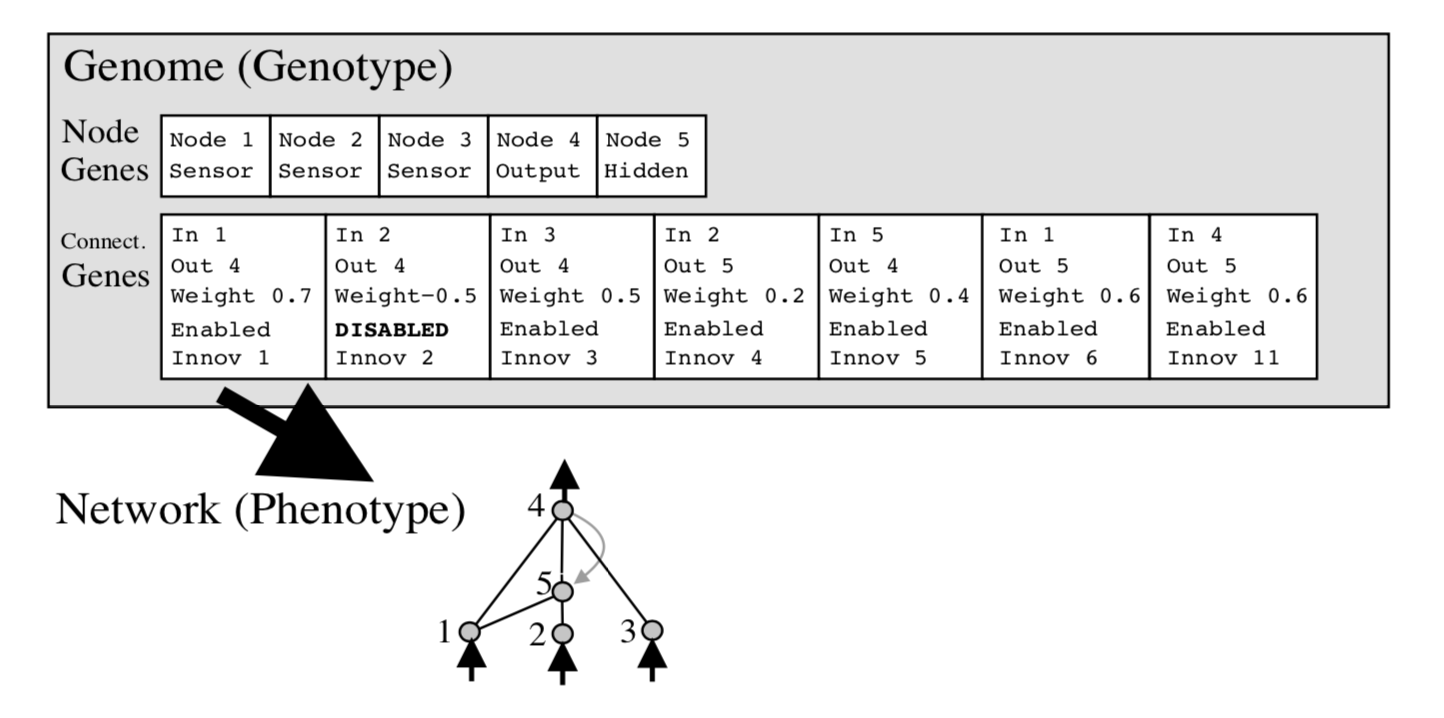
\includegraphics[width = \textwidth,left]{genome}
  \caption{ \tiny from Stanley, Kenneth O., and Risto Miikkulainen. (2002): 99-127.}
\end{figure}
\end{block}
\end{frame}



\begin{frame}{Crossover}
  \begin{block}{}
    \begin{figure}[htbp]
     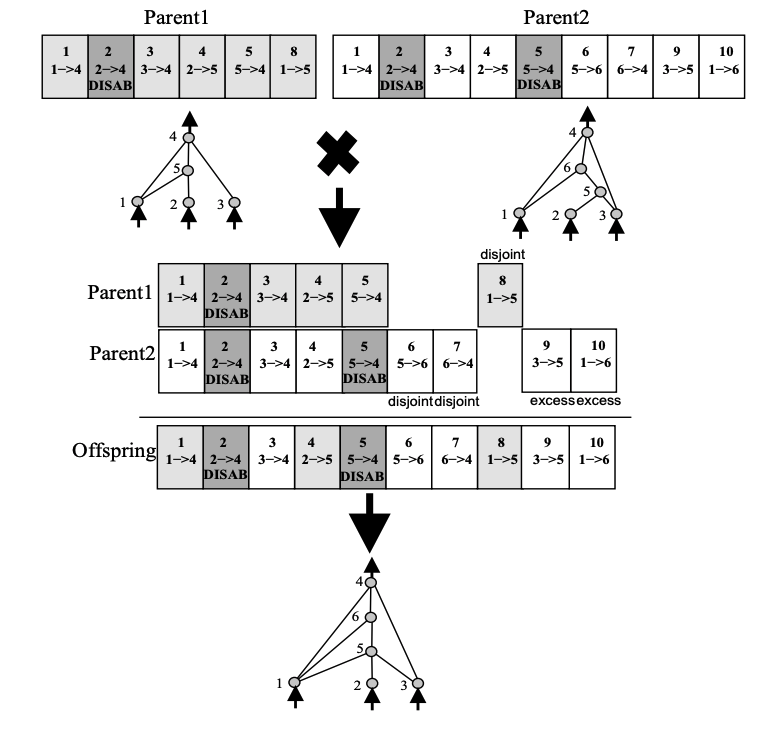
\includegraphics[width = .6\textwidth]{crossover}
     \caption{ \tiny from Stanley, Kenneth O., and Risto Miikkulainen. (2002): 99-127.}
    \end{figure}
    \end{block}
\end{frame}




%\subsection{parameterized policies}
\begin{frame}{mutation}
  \begin{block}{}
    \begin{figure}[htbp]
     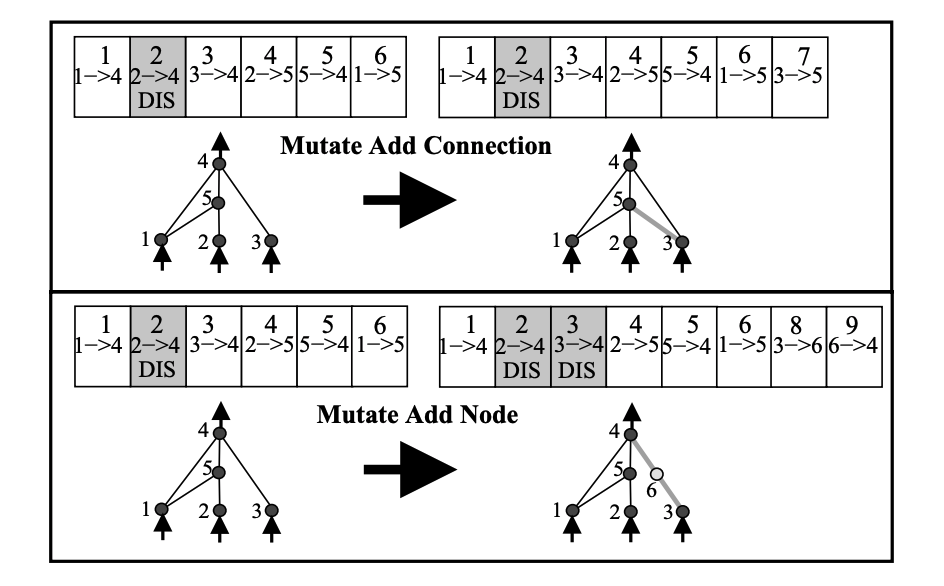
\includegraphics[width = .9\textwidth]{mutation}
     \caption{ \tiny from Stanley, Kenneth O., and Risto Miikkulainen. (2002): 99-127.}
    \end{figure}
    \end{block}
  
\end{frame}

\begin{frame}{}
  
  \begin{algorithm}[H]
    \scriptsize
    \caption{NEAT($S, A, p , m_n, m_l, g, e$)}
    \KwIn{$S$:set of all states, $A$:set of all actions, $p$:population size , $m_n$: rate of adding node, $m_l$: rate of adding link, $g$: generations, $e$: episodes;}
    \textbf{Initialize:} $P[] \leftarrow$ Init-Populations$(S,A,p)$ \;    
    \For{ $i \leftarrow 1 $ to $g$ }{\For{$j \leftarrow 1 $ to $e$}{
    $N, s, s^{\prime} \leftarrow $ Random($P$), null, INIT-STATE($S$)\;
    \While{Terminal-state?(s)}{
      $Q[] \leftarrow  $EVAL-NET$(N,s^{\prime})$\;
      $a^{\prime} \leftarrow \arg\max Q[j]$;  $\quad$
      $s, a \leftarrow s^{\prime}, a^{\prime}$;  $\quad$
      $r, s^{\prime} \leftarrow$ TAKE-ACTION$(a^{\prime})$\;
      $N.fitness \leftarrow N.fitness + r$
      }
      $N.episodes \leftarrow N.episodes + 1$
      }
    $P^{\prime} \leftarrow$ new array of size p\;
    \For{$j \leftarrow 1 $ to $p$}{
      $P^{\prime}[] \leftarrow$  Breed-Net$(P[])$\;
      \textbf{with-probability} $m_n$: ADD-Node-Mutation($P^{\prime}[j]$)\;
      \textbf{with-probability} $m_l$: ADD-link-Mutation($P^{\prime}[j]$)
    }
    $P[] \leftarrow P^{\prime}[]$
    }
    \end{algorithm}
\end{frame}

\section{method}
\begin{frame}{}
  \begin{algorithm}[H]
    \scriptsize
    {\tiny\caption{NEAT+Q($S, A, p , m_n, m_l, g, e$)}}
    \KwIn{$S$, $A$, $p$, $m_n$, $m_l$, $g$, $e$, $\alpha$, $\lambda$, $\gamma$, $\epsilon$}
    \textbf{Initialize:} $P[] \leftarrow$ Init-Populations$(S,A,p)$ \;    
    \For{ $i \leftarrow 1 $ to $g$ }{\For{$j \leftarrow 1 $ to $e$}{
    $N, s, s^{\prime} \leftarrow $ Random($P$), null, INIT-STATE($S$)\;
    \While{Terminal-state?(s)}{
      $Q[] \leftarrow  $EVAL-NET$(N,s^{\prime})$\;
      \textbf{With-prob}($\epsilon_{td}$) $a^{\prime} \leftarrow RANDOM(A)$\;
      \textbf{else:} $a^{\prime} \leftarrow \arg\max Q[j]$\;
      \If{$s \neq null $}
      {$BACKPROP(N,s,a,(r + \gamma \max_{j} Q[j])/ c, \alpha, \gamma, \lambda)$}
      $s, a \leftarrow s^{\prime}, a^{\prime}$\;
      $r, s^{\prime} \leftarrow$ TAKE-ACTION$(a^{\prime})$\;
      $N.fitness \leftarrow N.fitness + r$
      }
      $N.episodes \leftarrow N.episodes + 1$
      }
    Crossover and mutation

    }
    \end{algorithm}
\end{frame}





\begin{frame}{Boltzman Selection}
 Exploration probability:
  \begin{block}{}
    $$\Pr(\cdot| s) = \frac{e^{Q(s,\cdot)/\tau}}{\sum_{a\in A} e^{Q(s,a)/\tau}}$$
  \end{block}  
  Can we use it in network choosing? Yes.
  \begin{block}{}
    $$\Pr(\cdot) = \frac{e^{S(\cdot)/\tau}}{\sum_{q\in P} e^{S(q)/\tau}}$$
  \end{block}  
\end{frame}

\begin{frame}{}
  \begin{algorithm}[H]
    
    {\tiny\caption{Boltzman Selection($P, \tau$)}}
    \KwIn{$P:$ population, $\tau$: softmax temperature}
      \eIf{$\exists N \in P \ |\ N.episodes = 0 $}
      {return $N$}
      {$total \leftarrow \sum_{N \in P} e^{N.average / \tau}$\;
      \For{$N\in P$}{
        with-prob ($\frac{e^{N.average/\tau}}{total}$) return $N$
        else $total \leftarrow total - e^{N.average /\tau}$
      }
      }
      
    \end{algorithm}
\end{frame}

\begin{frame}
\begin{block}{Some Comparison}
   \begin{itemize}
      \item Online v.s. Offline
      \item Darwinian v.s. Lamarckian
      \item Annealing v.s. Without Annealing
   \end{itemize}
  \end{block}
\end{frame}

\begin{frame}{Experiments from the paper}
  \begin{itemize}
    \item mountain car
    \begin{figure}[htbp]
      \includegraphics[width = .5\textwidth]{mountaincar}
      \caption{from Sutton and Barto (1998)}
     \end{figure}
    \item Server job scheduling
  \end{itemize}
\end{frame}




\begin{frame}{Results}
  \begin{figure}[htbp]
    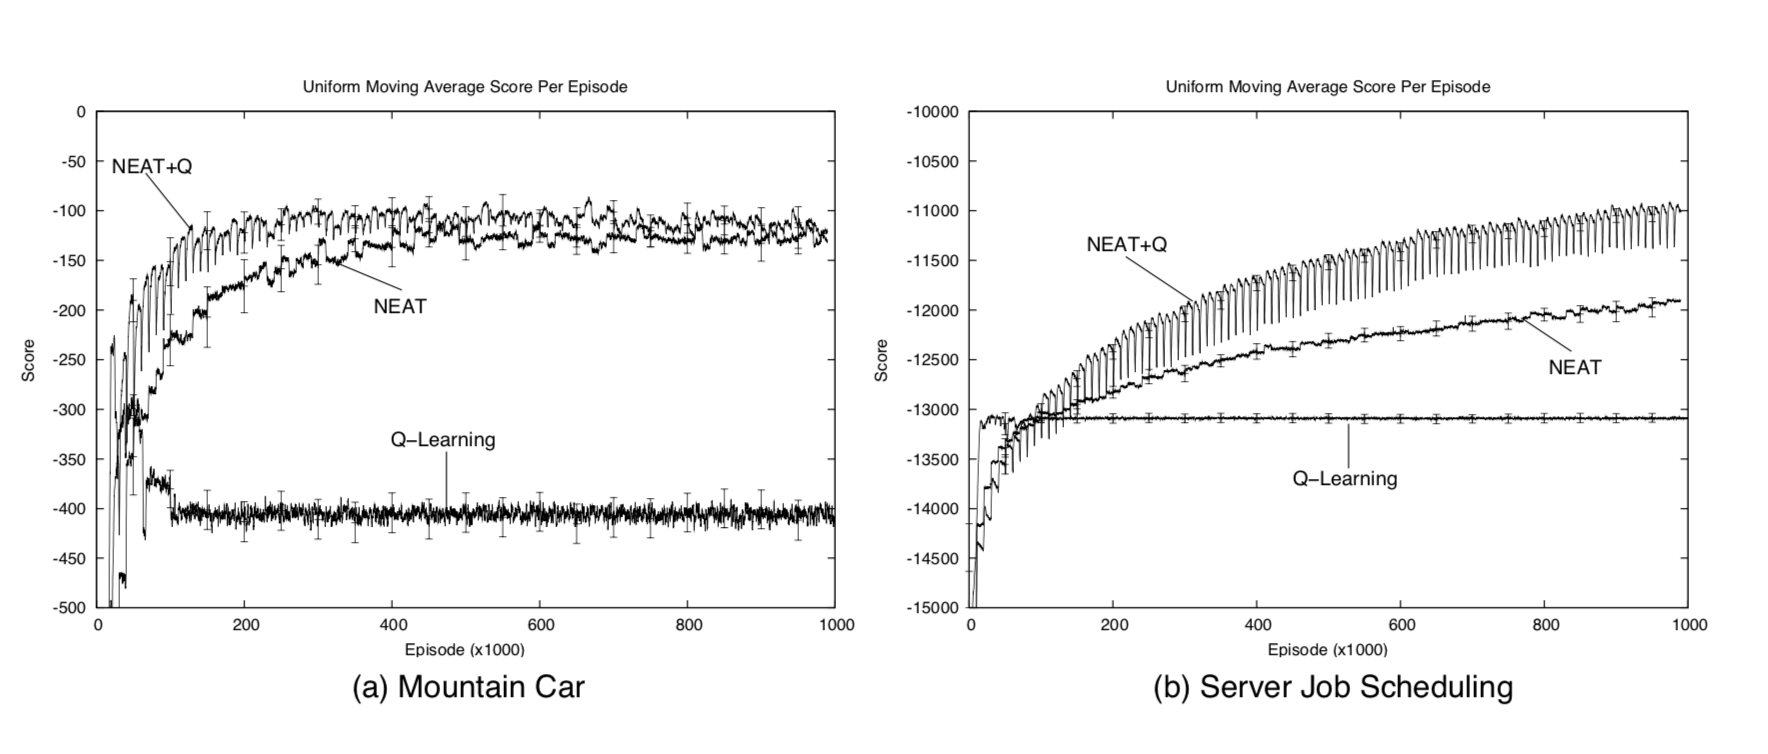
\includegraphics[width = 1.1\textwidth, left]{3result}
    \caption{from Whiteson, Shimon, and Peter Stone. (2006): 877-917. Figure 6}
   \end{figure}
  
\end{frame}

\begin{frame}{Results}
  \begin{figure}[htbp]
    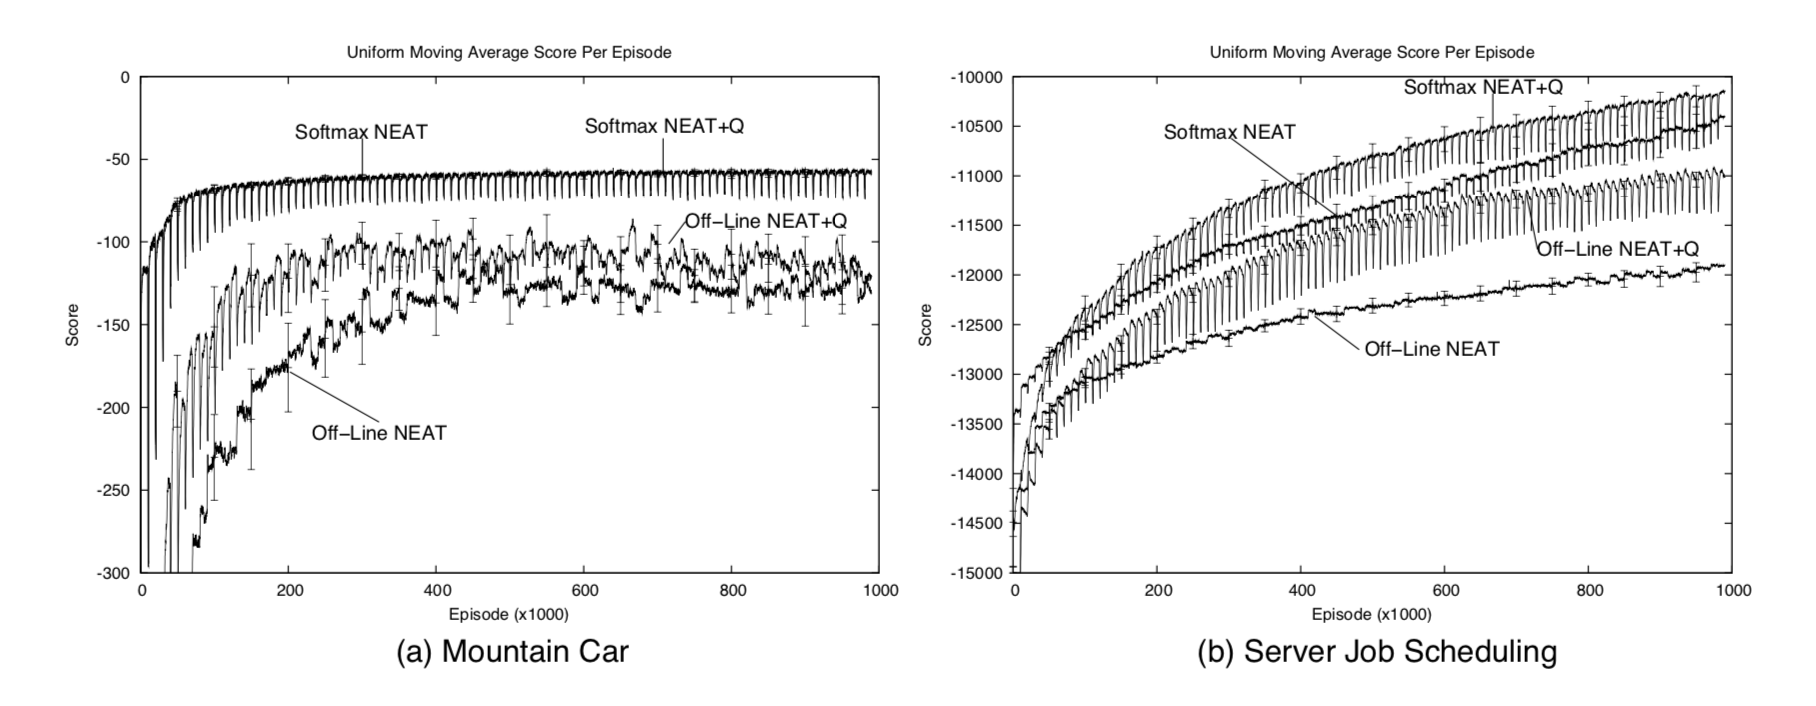
\includegraphics[width = 1.1\textwidth, left]{explorationneat}
    \caption{from Whiteson, Shimon, and Peter Stone. (2006): 877-917. Figure 7}
   \end{figure}
  
\end{frame}

\begin{frame}

  \begin{figure}[htbp]
    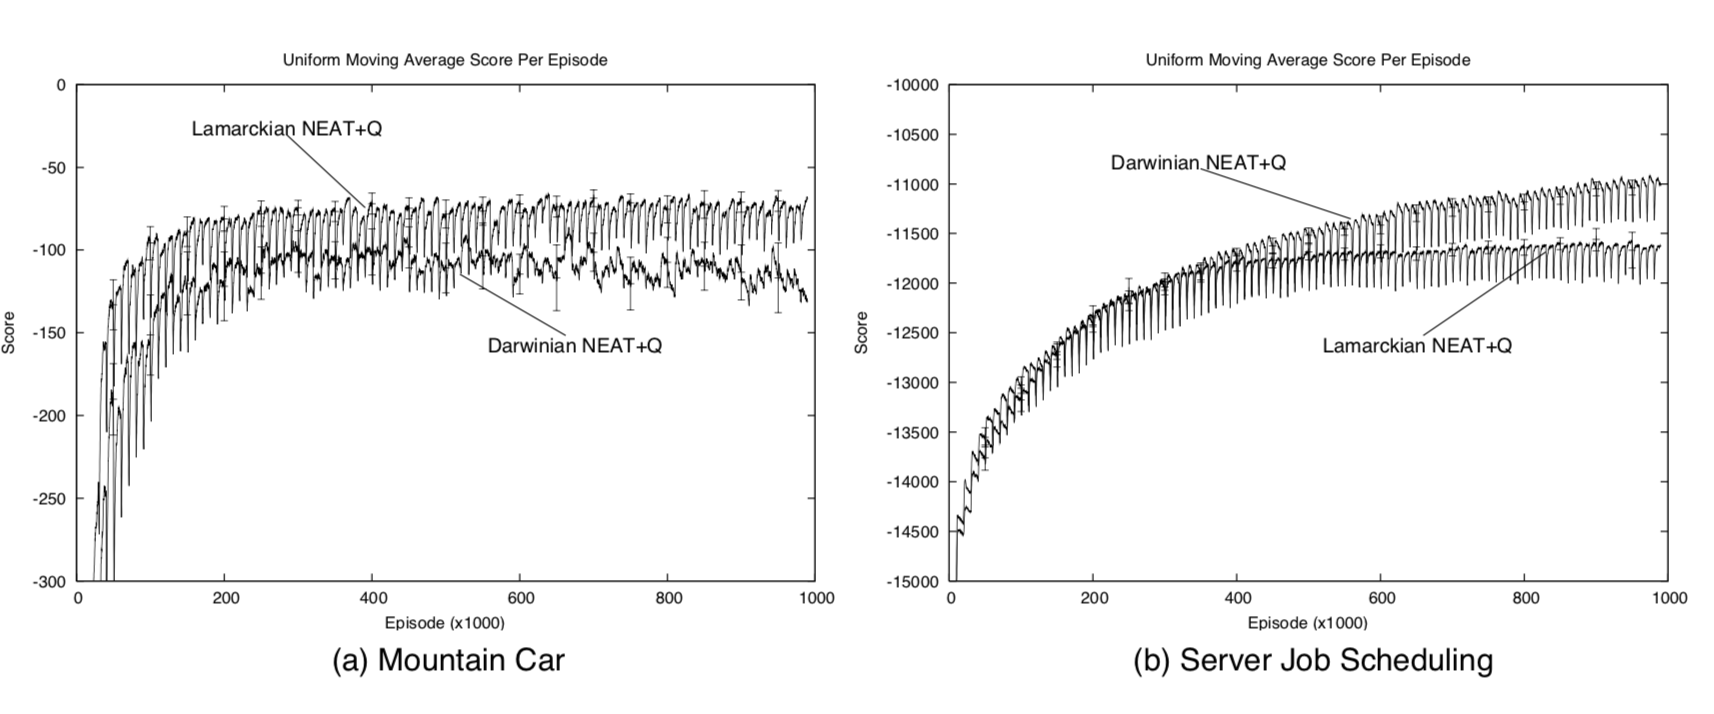
\includegraphics[width = 1.1\textwidth, left]{darwinian}
    \caption{from Whiteson, Shimon, and Peter Stone. (2006): 877-917. Figure 10}
   \end{figure}
\end{frame}

\begin{frame}

  \begin{figure}[htbp]
    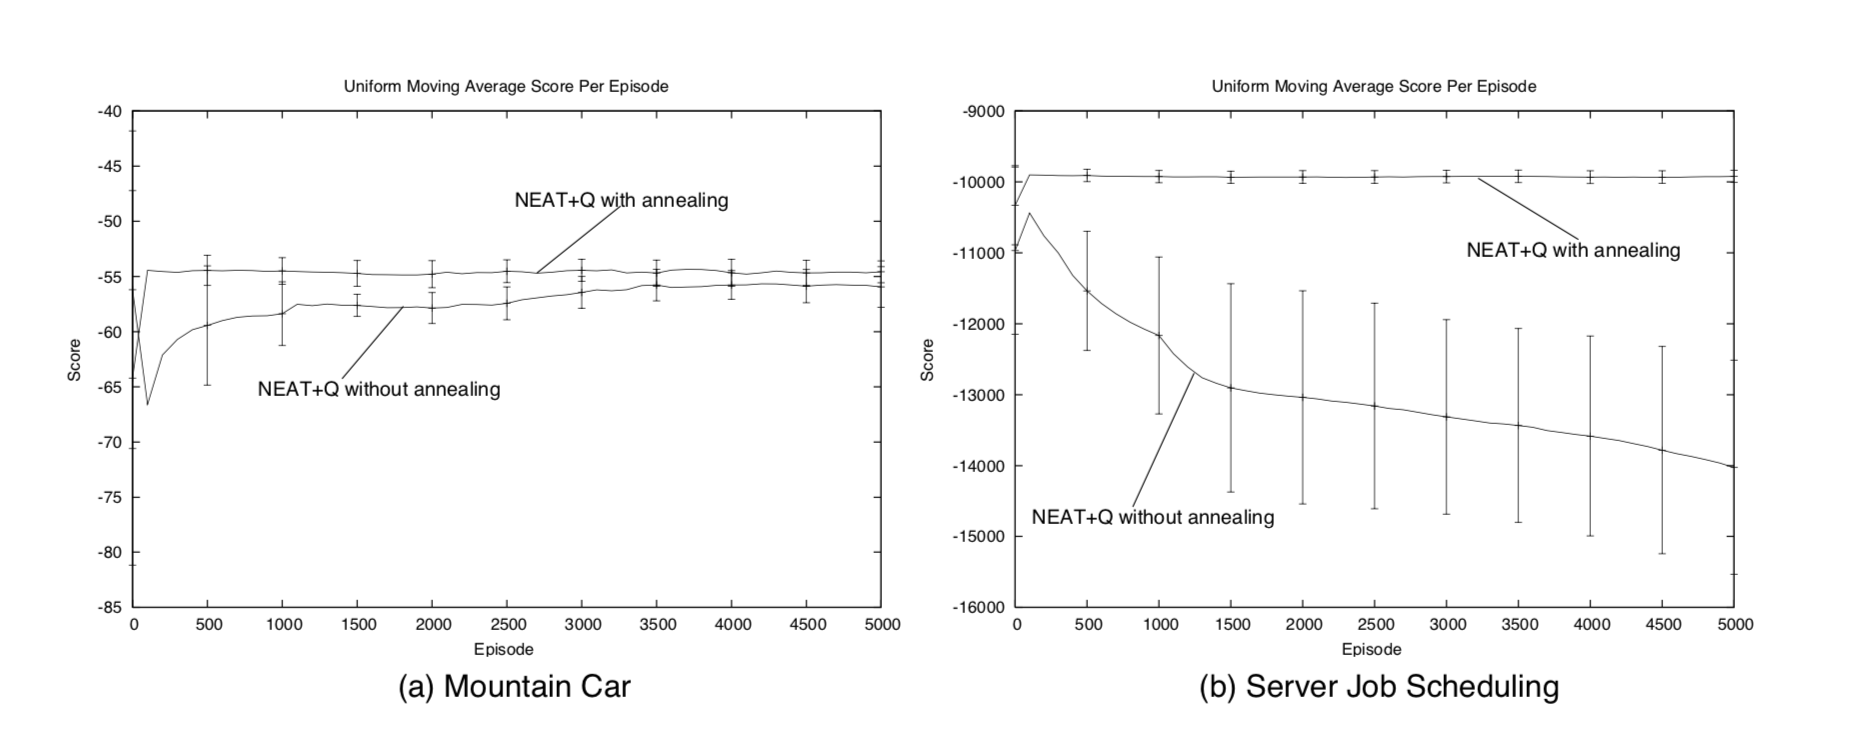
\includegraphics[width = 1.1\textwidth, left]{anneal}
    \caption{from Whiteson, Shimon, and Peter Stone. (2006): 877-917. Figure 11}
   \end{figure}
\end{frame}
\section{Experiments}
\begin{frame}{Experiments}
  \begin{block}{}
    Let's try it!
  \end{block}
  \begin{block}{}
    \begin{itemize}
      \item[(a)] Cartpole Balancing using NEAT and Q
      \item[(b)] test on Atari game Pacman on both NEAT and Q
    \end{itemize}
  \end{block}
  
  \end{frame}



\section{conclusion}

 \begin{frame}
  \begin{block}{Conclusion}
        \begin{itemize}
          \item NEAT outperform Q-learning in episodes, Generally, (NEAT+Q can perform better!)
          \item NEAT explore the function representation automatically.
          \item Some other Methods(DDQN and Duel QN, PG) can be combined with NEAT
          \item Non-stationary environment is challenging.
        \end{itemize}
      \end{block}
      \end{frame}

\begin{frame}
  \begin{block}{}
    \begin{equation}
      \mathbf{Thank} \ \mathbf{You} \mathbf{!} \nonumber
    \end{equation}
  \end{block}
\end{frame}


\end{document}
